\documentclass[10pt, a4paper]{article}\usepackage[]{graphicx}\usepackage[]{color}
%% maxwidth is the original width if it is less than linewidth
%% otherwise use linewidth (to make sure the graphics do not exceed the margin)
\makeatletter
\def\maxwidth{ %
  \ifdim\Gin@nat@width>\linewidth
    \linewidth
  \else
    \Gin@nat@width
  \fi
}
\makeatother

\definecolor{fgcolor}{rgb}{0.345, 0.345, 0.345}
\newcommand{\hlnum}[1]{\textcolor[rgb]{0.686,0.059,0.569}{#1}}%
\newcommand{\hlstr}[1]{\textcolor[rgb]{0.192,0.494,0.8}{#1}}%
\newcommand{\hlcom}[1]{\textcolor[rgb]{0.678,0.584,0.686}{\textit{#1}}}%
\newcommand{\hlopt}[1]{\textcolor[rgb]{0,0,0}{#1}}%
\newcommand{\hlstd}[1]{\textcolor[rgb]{0.345,0.345,0.345}{#1}}%
\newcommand{\hlkwa}[1]{\textcolor[rgb]{0.161,0.373,0.58}{\textbf{#1}}}%
\newcommand{\hlkwb}[1]{\textcolor[rgb]{0.69,0.353,0.396}{#1}}%
\newcommand{\hlkwc}[1]{\textcolor[rgb]{0.333,0.667,0.333}{#1}}%
\newcommand{\hlkwd}[1]{\textcolor[rgb]{0.737,0.353,0.396}{\textbf{#1}}}%

\usepackage{framed}
\makeatletter
\newenvironment{kframe}{%
 \def\at@end@of@kframe{}%
 \ifinner\ifhmode%
  \def\at@end@of@kframe{\end{minipage}}%
  \begin{minipage}{\columnwidth}%
 \fi\fi%
 \def\FrameCommand##1{\hskip\@totalleftmargin \hskip-\fboxsep
 \colorbox{shadecolor}{##1}\hskip-\fboxsep
     % There is no \\@totalrightmargin, so:
     \hskip-\linewidth \hskip-\@totalleftmargin \hskip\columnwidth}%
 \MakeFramed {\advance\hsize-\width
   \@totalleftmargin\z@ \linewidth\hsize
   \@setminipage}}%
 {\par\unskip\endMakeFramed%
 \at@end@of@kframe}
\makeatother

\definecolor{shadecolor}{rgb}{.97, .97, .97}
\definecolor{messagecolor}{rgb}{0, 0, 0}
\definecolor{warningcolor}{rgb}{1, 0, 1}
\definecolor{errorcolor}{rgb}{1, 0, 0}
\newenvironment{knitrout}{}{} % an empty environment to be redefined in TeX

\usepackage{alltt}
\usepackage{fancyhdr}
\usepackage{bookman}
\usepackage{amsthm}
\usepackage{natbib}

\pagestyle{fancy} \rhead[RH-even]{}
\setlength{\oddsidemargin}{0pt} \setlength{\evensidemargin}{0pt}
\setlength{\textwidth}{450pt}
\newcommand{\markforthis}[1]{\nolinebreak\hfill [#1]}
\IfFileExists{upquote.sty}{\usepackage{upquote}}{}
\begin{document}


\begin{titlepage}


\begin{center}
\vspace* {0.70 in}

\noindent\makebox[\linewidth]{\rule{\paperwidth}{0.4pt}}

\huge{Vignette for the {\tt MRSea} Package (v0.2.0)}\\[0.5 cm]
%\Large{University of St. Andrews}\\
\Large{Statistical Modelling of bird and cetacean distributions in offshore renewables development areas}\\
\vspace{0.3 in}
\today

\noindent\makebox[\linewidth]{\rule{\paperwidth}{0.4pt}}


\vspace{1 in}
\Large{Lindesay Scott-Hayward}\\
\Large{Cornelia Oedekoven}\\
\Large{Monique Mackenzie}\\
\Large{Cameron Walker}\\[0.5 cm]


\vspace{1.6 in}
\begin{center}
\large{This vignette constitutes work carried out at the Centre for Research into Ecological and Environmental Modelling (CREEM) at the University of St. Andrews.}
\end{center}


\thispagestyle{empty}

\end{center}

\end{titlepage}

\vspace{0.3cm}
\textbf{Please reference this document as:}
\noindent Scott-Hayward, L.A.S., Oedekoven, C.S., Mackenzie, M.L. and Walker, C.G. (2015). Vignette for the MRSea Package v0.2.0: Statistical Modelling of bird and cetacean distributions in offshore renewables development areas. Centre for Research into Ecological and Environmental Modelling, University of St Andrews.



%


%~~~~~~~~~~~~~~~~~~~~~~~~
\section{Introduction}
The {\tt MRSea} package was developed for analysing data that was collected for assessing potential impacts of renewable developments on marine wildlife, although the methods are applicable to other studies as well. This vignette gives an updated example of the code for version 0.2.0.  For additional information regarding methods, see Mackenzie, et al. (2013) and Scott-Hayward, et al. (2013).  The user should be familiar with generalised linear models and their assumptions and model selection. The {\tt MRSea} package primarily allows spatially adaptive model selection for both one and two dimensional covariates using the functions {\tt runSALSA1D\_withremoval} and {\tt runSALSA2D}, which implement the methods of Walker, et al. (2010) and Scott-Hayward, et al. (2013). Other functions include diagnostics (to assess residual correlation: {\tt runACF}, smooth relationships: {\tt runPartialPlots} and model selection (ANOVA) for a Generalised Estimating Equation used when residual correlation is present: {\tt getPvalues}) and inference ({\tt do.bootstrap.cress}). 


\begin{figure}[!h]
{\centering 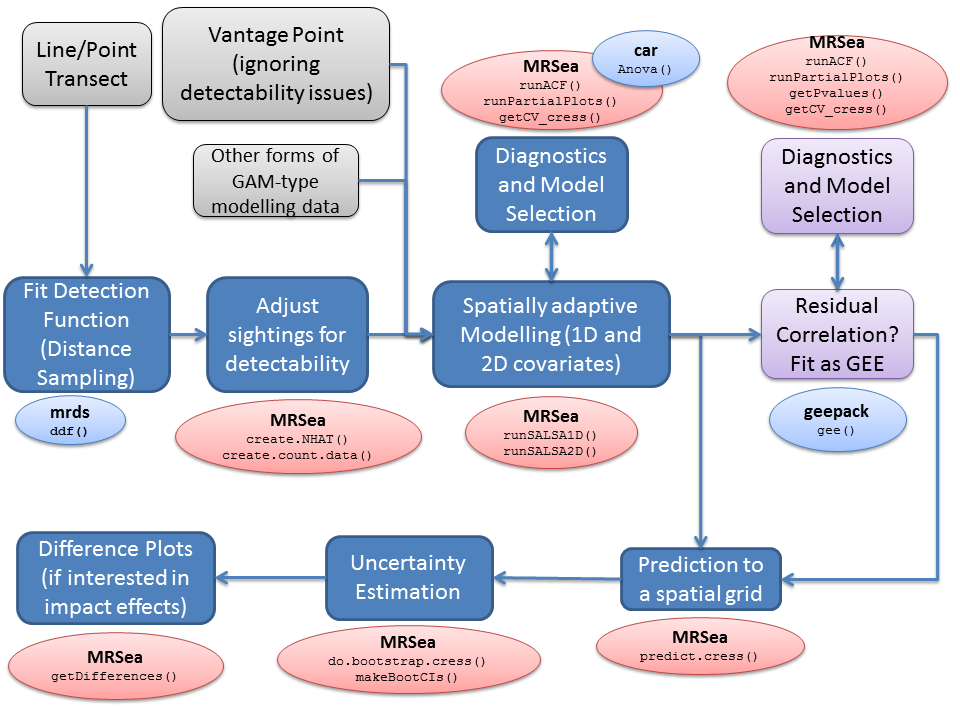
\includegraphics[width=0.8\maxwidth]{MRSea_workflow.png} 
\caption{Example of the modelling process using MRSea.  Packages with functions to run certain parts are given in oval boxes.  To complete the modelling process, other packages may be used at certain stages Hojsgaard, et al. (2006); Laake, et al. (2014); Fox, et al. (2011).  These are coded light blue, whilst MRSea functions are in red.  GEE (far right), stands for Generalised Estimating Equations.}
}
\end{figure}

\vspace{0.3cm}
A full description of each of the functions within the {\tt MRSea} package can be found in the reference manual at: \\
\href{http://creem2.st-and.ac.uk/software.aspx}{http://creem2.st-and.ac.uk/software.aspx}.  The manual and this document use version 0.2.0 of MRSea.

\vspace{0.3cm}

\begin{enumerate}

\section{Distance sampling using the {\tt mrds} library}

\item Load data and fit detection function (Distance Sampling)
\begin{knitrout}
\definecolor{shadecolor}{rgb}{0.969, 0.969, 0.969}\color{fgcolor}\begin{kframe}
\begin{alltt}
\hlkwd{require}\hlstd{(MRSea)}
\hlcom{# we will use the dataset with a known re-distribution of animals}
\hlkwd{data}\hlstd{(dis.data.re)}
\hlstd{dis.data}\hlkwb{<-}\hlstd{dis.data.re}
\hlkwd{require}\hlstd{(mrds)} \hlcom{# distance sampling package}
\hlstd{result} \hlkwb{<-} \hlkwd{ddf}\hlstd{(}\hlkwc{dsmodel}\hlstd{=}\hlopt{~}\hlkwd{mcds}\hlstd{(}\hlkwc{key}\hlstd{=}\hlstr{"hn"}\hlstd{,} \hlkwc{formula}\hlstd{=}\hlopt{~}\hlnum{1}\hlstd{),}
              \hlkwc{data} \hlstd{= dis.data,} \hlkwc{method}\hlstd{=}\hlstr{"ds"}\hlstd{,}
              \hlkwc{meta.data}\hlstd{=}\hlkwd{list}\hlstd{(}\hlkwc{width}\hlstd{=}\hlnum{250}\hlstd{))}
\end{alltt}
\end{kframe}
\end{knitrout}

\item Adjust sightings for detectability 
\begin{knitrout}
\definecolor{shadecolor}{rgb}{0.969, 0.969, 0.969}\color{fgcolor}\begin{kframe}
\begin{alltt}
\hlcom{# create.NHAT and create.count.data are MRSea functions to adjust the }
\hlcom{# sightings for the detection function estimated above.}
\hlstd{dis.data} \hlkwb{<-} \hlkwd{create.NHAT}\hlstd{(dis.data,result)}
\hlstd{count.data} \hlkwb{<-} \hlkwd{create.count.data}\hlstd{(dis.data)}
\end{alltt}
\end{kframe}
\end{knitrout}

\item Try a simple model
\begin{knitrout}
\definecolor{shadecolor}{rgb}{0.969, 0.969, 0.969}\color{fgcolor}\begin{kframe}
\begin{alltt}
\hlstd{data} \hlkwb{<-} \hlstd{count.data}
\hlstd{data}\hlopt{$}\hlstd{response} \hlkwb{<-} \hlkwd{round}\hlstd{(data}\hlopt{$}\hlstd{NHAT)}
\hlkwd{attach}\hlstd{(data)}
\hlstd{fullModel} \hlkwb{<-} \hlkwd{glm}\hlstd{(response} \hlopt{~} \hlkwd{as.factor}\hlstd{(season)} \hlopt{+} \hlkwd{as.factor}\hlstd{(impact)} \hlopt{+}
                   \hlstd{depth} \hlopt{+} \hlstd{x.pos} \hlopt{+} \hlstd{y.pos,} \hlkwc{family} \hlstd{= poisson,} \hlkwc{data} \hlstd{= data)}
\end{alltt}
\end{kframe}
\end{knitrout}

\item Try a model with a smooth term for depth
\begin{knitrout}
\definecolor{shadecolor}{rgb}{0.969, 0.969, 0.969}\color{fgcolor}\begin{kframe}
\begin{alltt}
\hlcom{#knots <- mean(depth) # must be specified as an object}
\hlkwd{require}\hlstd{(splines)}
\hlstd{fullModel} \hlkwb{<-} \hlkwd{glm}\hlstd{(response} \hlopt{~} \hlkwd{as.factor}\hlstd{(season)} \hlopt{+} \hlkwd{as.factor}\hlstd{(impact)} \hlopt{+}
                   \hlkwd{bs}\hlstd{(depth,} \hlkwc{knots} \hlstd{=} \hlkwd{mean}\hlstd{(depth))} \hlopt{+} \hlstd{x.pos} \hlopt{+} \hlstd{y.pos,}
                 \hlkwc{family} \hlstd{= poisson,}\hlkwc{data} \hlstd{= data)}
\end{alltt}
\end{kframe}
\end{knitrout}

\item SALSA1D requires that {\tt foldid} is a column in the data set so that $k$-fold Cross-Validation (CV) may be used.  The user may specify how many folds (5 or 10 is usual) and whether or not the data has a blocking structure.  If the data are correlated then when selecting folds for the CV, the blocks must not be split up.


For correlated data:
\begin{knitrout}
\definecolor{shadecolor}{rgb}{0.969, 0.969, 0.969}\color{fgcolor}\begin{kframe}
\begin{alltt}
\hlcom{# for correlated data:}
\hlstd{data}\hlopt{$}\hlstd{blockid} \hlkwb{<-} \hlkwd{paste}\hlstd{(data}\hlopt{$}\hlstd{transect.id, data}\hlopt{$}\hlstd{season, data}\hlopt{$}\hlstd{impact,}\hlkwc{sep} \hlstd{=} \hlstr{""}\hlstd{)}
\hlstd{data}\hlopt{$}\hlstd{foldid} \hlkwb{<-} \hlkwd{getCVids}\hlstd{(}\hlkwc{data} \hlstd{= data,} \hlkwc{folds} \hlstd{=} \hlnum{5}\hlstd{,} \hlkwc{block} \hlstd{=} \hlstr{'blockid'}\hlstd{)}
\end{alltt}
\end{kframe}
\end{knitrout}

or uncorrelated data:
\begin{knitrout}
\definecolor{shadecolor}{rgb}{0.969, 0.969, 0.969}\color{fgcolor}\begin{kframe}
\begin{alltt}
\hlcom{# for uncorrelated data@}
\hlstd{data}\hlopt{$}\hlstd{foldid}\hlkwb{<-} \hlkwd{getCVids}\hlstd{(}\hlkwc{data}\hlstd{=data,} \hlkwc{folds}\hlstd{=}\hlnum{5}\hlstd{)}
\end{alltt}
\end{kframe}
\end{knitrout}

\section{Selection of 1D Covariates}
Run SALSA1D to select what covariates are included and whether or not they are smooth.  SALSA selects the smoothness of each term (number and location of knots) and CV is used to choose between the best smooth term, a linear term or no term at all.  To not allow the removal process the user may set {\tt removal = FALSE} as a parameter in the function {\tt runSALSA1D\_withremoval}.

\item Specify the parameters required:

\begin{knitrout}
\definecolor{shadecolor}{rgb}{0.969, 0.969, 0.969}\color{fgcolor}\begin{kframe}
\begin{alltt}
\hlstd{salsa1dlist} \hlkwb{<-} \hlkwd{list}\hlstd{(}\hlkwc{fitnessMeasure} \hlstd{=} \hlstr{"AICh"}\hlstd{,} \hlkwc{minKnots_1d} \hlstd{=} \hlnum{2}\hlstd{,}\hlkwc{maxKnots_1d} \hlstd{=} \hlnum{5}\hlstd{,}
                    \hlkwc{startKnots_1d} \hlstd{=} \hlnum{1}\hlstd{,} \hlkwc{degree} \hlstd{=} \hlnum{2}\hlstd{,} \hlkwc{maxIterations} \hlstd{=} \hlnum{10}\hlstd{,}
                    \hlkwc{gaps} \hlstd{=} \hlkwd{c}\hlstd{(}\hlnum{1}\hlstd{))}
\end{alltt}
\end{kframe}
\end{knitrout}

\item If you wish to make predictions once the model is fitted, then a prediction grid should be created and specified.  This is because the splines fitted here (B-splines) are unable to make predictions outside of the range they were created.  For example, if the data range for depth is smaller than the range of depths in the prediction data, predictions cannot be made.  
\begin{knitrout}
\definecolor{shadecolor}{rgb}{0.969, 0.969, 0.969}\color{fgcolor}\begin{kframe}
\begin{alltt}
\hlkwd{data}\hlstd{(predict.data.re)}  \hlcom{# contains predict.data}
\hlcom{# This is a spatial grid for making predictions.  All covariates in }
\hlcom{# final model must be in this data frame and the naming must be the }
\hlcom{# same as for the data}
\hlstd{predictData} \hlkwb{<-} \hlstd{predict.data.re}
\hlkwd{range}\hlstd{(data}\hlopt{$}\hlstd{depth)}
\end{alltt}
\begin{verbatim}
## [1] -28.608  -0.411
\end{verbatim}
\begin{alltt}
\hlkwd{range}\hlstd{(predictData}\hlopt{$}\hlstd{depth)}
\end{alltt}
\begin{verbatim}
## [1] -28.61  -0.20
\end{verbatim}
\end{kframe}
\end{knitrout}

Here the range of the predictions is slightly wider than the range of the data, so we will specify {\tt predictData} when running SALSA.

\item Set up the initial model with factor covariates and the offset term (if required), and run SALSA.
\begin{knitrout}
\definecolor{shadecolor}{rgb}{0.969, 0.969, 0.969}\color{fgcolor}\begin{kframe}
\begin{alltt}
\hlstd{initialModel} \hlkwb{<-} \hlkwd{glm}\hlstd{(response} \hlopt{~} \hlkwd{as.factor}\hlstd{(season)} \hlopt{+} \hlkwd{as.factor}\hlstd{(impact)}
                    \hlopt{+} \hlkwd{offset}\hlstd{(}\hlkwd{log}\hlstd{(area)),} \hlkwc{family} \hlstd{=} \hlstr{"quasipoisson"}\hlstd{,}
                    \hlkwc{data} \hlstd{= data)}
\end{alltt}
\end{kframe}
\end{knitrout}



\begin{knitrout}
\definecolor{shadecolor}{rgb}{0.969, 0.969, 0.969}\color{fgcolor}\begin{kframe}
\begin{alltt}
\hlcom{# run SALSA}
\hlstd{salsa1dOutput} \hlkwb{<-} \hlkwd{runSALSA1D_withremoval}\hlstd{(initialModel, salsa1dlist,} \hlkwd{c}\hlstd{(}\hlstr{"depth"}\hlstd{),}
                      \hlkwc{predictionData}\hlstd{=predictData,} \hlkwc{datain}\hlstd{=data,} \hlkwc{removal}\hlstd{=}\hlnum{TRUE}\hlstd{)}
\end{alltt}
\end{kframe}
\end{knitrout}

\begin{knitrout}
\definecolor{shadecolor}{rgb}{0.969, 0.969, 0.969}\color{fgcolor}\begin{kframe}
\begin{alltt}
\hlcom{# How many knots were chosen for depth?}
\hlstd{salsa1dOutput}\hlopt{$}\hlstd{splineParams[[}\hlnum{2}\hlstd{]]}\hlopt{$}\hlstd{knots}
\end{alltt}
\begin{verbatim}
## [1] -16.62
\end{verbatim}
\begin{alltt}
\hlstd{splineParams}\hlkwb{<-}\hlstd{salsa1dOutput}\hlopt{$}\hlstd{splineParams}
\hlcom{# ~~~~~~~~~~~~~~~~~~~~~~~}
\end{alltt}
\end{kframe}
\end{knitrout}


\section{Selection of flexibility for 2D smooth term}

\item Create a grid of knots that will be used as possible knot locations.  This may take while and could be different every time you run it so I suggest saving the knotgrid as a file.

\begin{knitrout}
\definecolor{shadecolor}{rgb}{0.969, 0.969, 0.969}\color{fgcolor}\begin{kframe}
\begin{alltt}
\hlstd{knotgrid}\hlkwb{<-} \hlkwd{getKnotgrid}\hlstd{(}\hlkwc{coordData} \hlstd{=} \hlkwd{cbind}\hlstd{(data}\hlopt{$}\hlstd{x.pos, data}\hlopt{$}\hlstd{y.pos))}
\hlcom{#}
\hlcom{# write.csv(knotgrid, file='knotgrid_fullanalysis.csv', row.names=F)}
\hlcom{# ~~~~~~~~~~~~~~~~~~~~~~~}
\end{alltt}
\end{kframe}

{\centering 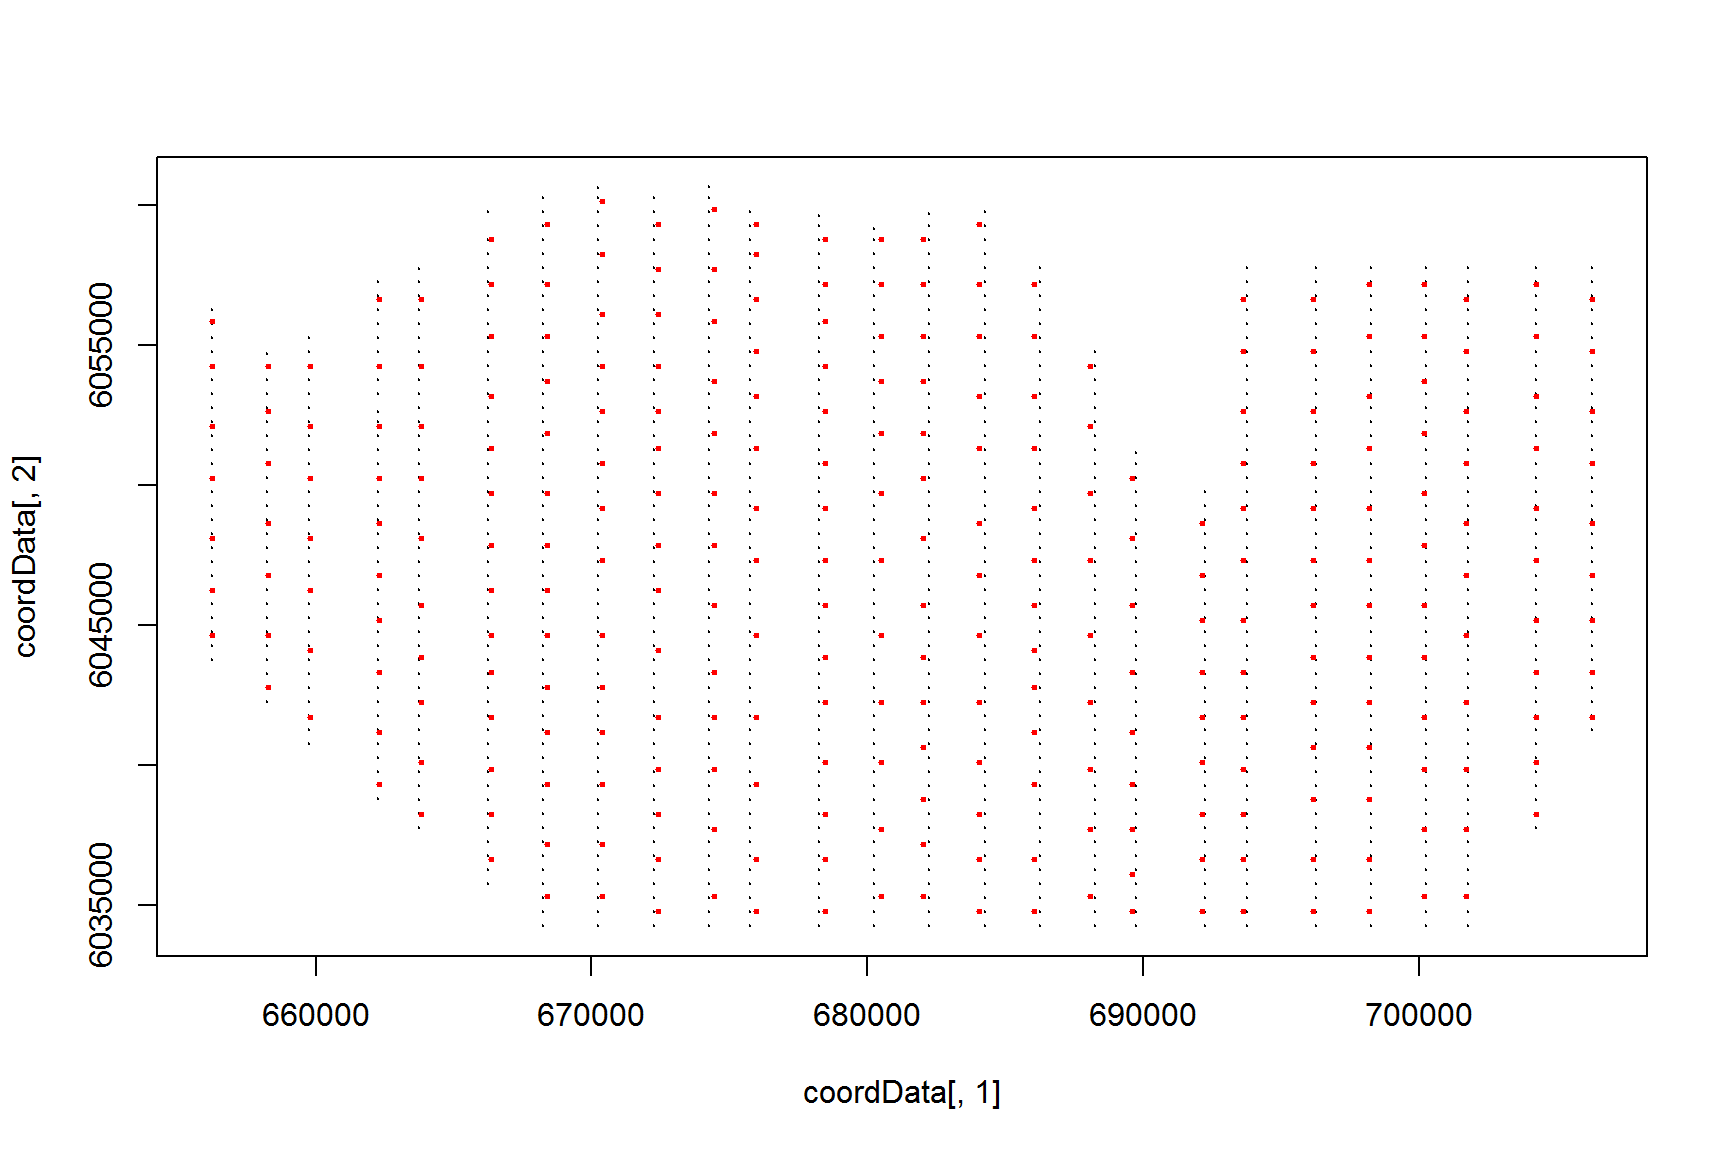
\includegraphics[width=0.9\linewidth]{figure/knotgrid} 

}



\end{knitrout}
The black points in the figure are the data and the red points, the candidate knot locations.

\item Set up parameters for SALSA2D.  Distance matrices and the range parameter.  The default setting of 10 radii should be fine for general use.  Choose a fit statistic, min, max and start knots.

\begin{knitrout}
\definecolor{shadecolor}{rgb}{0.969, 0.969, 0.969}\color{fgcolor}\begin{kframe}
\begin{alltt}
\hlcom{# make distance matrices for datatoknots and knottoknots}
\hlstd{distMats} \hlkwb{<-} \hlkwd{makeDists}\hlstd{(}\hlkwd{cbind}\hlstd{(data}\hlopt{$}\hlstd{x.pos, data}\hlopt{$}\hlstd{y.pos),} \hlkwd{na.omit}\hlstd{(knotgrid))}

\hlstd{r_seq} \hlkwb{<-} \hlkwd{getRadiiChoices}\hlstd{(}\hlkwc{numberofradii}\hlstd{=}\hlnum{10}\hlstd{,} \hlkwc{distMatrix}\hlstd{=distMats}\hlopt{$}\hlstd{dataDist)}

\hlcom{# ~~~~~~~~~~~~~~~~~~~~~~~}

\hlcom{# make parameter set for running salsa2d}
\hlstd{salsa2dlist}\hlkwb{<-}\hlkwd{list}\hlstd{(}\hlkwc{fitnessMeasure} \hlstd{=} \hlstr{'AICh'}\hlstd{,} \hlkwc{knotgrid} \hlstd{= knotgrid,}
                  \hlkwc{knotdim}\hlstd{=}\hlkwd{c}\hlstd{(}\hlnum{100}\hlstd{,}\hlnum{100}\hlstd{),} \hlkwc{startKnots}\hlstd{=}\hlnum{10}\hlstd{,} \hlkwc{minKnots}\hlstd{=}\hlnum{4}\hlstd{,}
                  \hlkwc{maxKnots}\hlstd{=}\hlnum{12}\hlstd{,} \hlkwc{r_seq}\hlstd{=r_seq,} \hlkwc{gap}\hlstd{=}\hlnum{4000}\hlstd{,}
                  \hlkwc{interactionTerm}\hlstd{=}\hlstr{"as.factor(impact)"}\hlstd{)}
\end{alltt}
\end{kframe}
\end{knitrout}

\item Run SALSA2D to find the appropriate number and location of knots for the 2D smooth term of {\tt x.pos} and {\tt y.pos}.


\begin{knitrout}
\definecolor{shadecolor}{rgb}{0.969, 0.969, 0.969}\color{fgcolor}\begin{kframe}
\begin{alltt}
\hlstd{salsa2dOutput_k6}\hlkwb{<-}\hlkwd{runSALSA2D}\hlstd{(salsa1dOutput}\hlopt{$}\hlstd{bestModel, salsa2dlist,}
                             \hlkwc{d2k}\hlstd{=distMats}\hlopt{$}\hlstd{dataDist,} \hlkwc{k2k}\hlstd{=distMats}\hlopt{$}\hlstd{knotDist,}
                             \hlkwc{splineParams}\hlstd{=splineParams)}
\end{alltt}
\end{kframe}
\end{knitrout}
\item Update relevent SALSA parameters in your workspace (this is important for updating the model or making predictions).

\begin{knitrout}
\definecolor{shadecolor}{rgb}{0.969, 0.969, 0.969}\color{fgcolor}\begin{kframe}
\begin{alltt}
\hlstd{splineParams}\hlkwb{<-}\hlstd{salsa2dOutput_k6}\hlopt{$}\hlstd{splineParams}
\hlcom{# specify parameters for local radial function:}
\hlstd{radiusIndices} \hlkwb{<-} \hlstd{splineParams[[}\hlnum{1}\hlstd{]]}\hlopt{$}\hlstd{radiusIndices}
\hlstd{dists} \hlkwb{<-} \hlstd{splineParams[[}\hlnum{1}\hlstd{]]}\hlopt{$}\hlstd{dist}
\hlstd{radii} \hlkwb{<-} \hlstd{splineParams[[}\hlnum{1}\hlstd{]]}\hlopt{$}\hlstd{radii}
\hlstd{aR} \hlkwb{<-} \hlstd{splineParams[[}\hlnum{1}\hlstd{]]}\hlopt{$}\hlstd{invInd[splineParams[[}\hlnum{1}\hlstd{]]}\hlopt{$}\hlstd{knotPos]}
\end{alltt}
\end{kframe}
\end{knitrout}

\item Are the residuals correlated? Make a suitable blocking structure, within which residuals are expected to be correlated but between which they are independent.  Use {\tt runACF} to assess the blocking structure.

\begin{knitrout}
\definecolor{shadecolor}{rgb}{0.969, 0.969, 0.969}\color{fgcolor}\begin{kframe}
\begin{alltt}
\hlstd{data}\hlopt{$}\hlstd{blockid}\hlkwb{<-}\hlkwd{paste}\hlstd{(data}\hlopt{$}\hlstd{transect.id, data}\hlopt{$}\hlstd{season, data}\hlopt{$}\hlstd{impact,} \hlkwc{sep}\hlstd{=}\hlstr{''}\hlstd{)}
\hlkwd{runACF}\hlstd{(}\hlkwc{block} \hlstd{= data}\hlopt{$}\hlstd{blockid,} \hlkwc{model} \hlstd{= salsa2dOutput_k6}\hlopt{$}\hlstd{bestModel)}
\end{alltt}
\end{kframe}
\end{knitrout}



\begin{figure}
{\centering \includegraphics[width=0.6\maxwidth]{figure/unnamed-chunk-13} 
\caption{ACF plot showing correlation in each block (grey lines), and the mean correlation by lag across blocks (red line).}
}
\end{figure}


Update the model to run a GEE to account for the correlation in the residuals (seen in the ACF plot).  The point estimates do not change as an independent working correlation structure is used, however, the standard errors are now appropriate and may be used for inference.

\begin{knitrout}
\definecolor{shadecolor}{rgb}{0.969, 0.969, 0.969}\color{fgcolor}\begin{kframe}
\begin{alltt}
\hlcom{# Re-fit the chosen model as a GEE (based on SALSA knot placement) and }
\hlcom{# GEE p-values}
\hlkwd{require}\hlstd{(geepack)}
\hlstd{geeModel}\hlkwb{<-} \hlkwd{geeglm}\hlstd{(}\hlkwd{formula}\hlstd{(salsa2dOutput_k6}\hlopt{$}\hlstd{bestModel),} \hlkwc{data}\hlstd{=data,}
                  \hlkwc{family}\hlstd{=poisson,} \hlkwc{id}\hlstd{=blockid)}
\end{alltt}
\end{kframe}
\end{knitrout}

\item Check for model selection
\begin{knitrout}
\definecolor{shadecolor}{rgb}{0.969, 0.969, 0.969}\color{fgcolor}\begin{kframe}
\begin{alltt}
\hlkwd{getPvalues}\hlstd{(}\hlkwc{model} \hlstd{= geeModel,} \hlkwc{varlist} \hlstd{=} \hlstr{'depth'}\hlstd{,}
           \hlkwc{factorlist} \hlstd{=} \hlkwd{c}\hlstd{(}\hlstr{'season'}\hlstd{,} \hlstr{'impact'}\hlstd{))}
\end{alltt}
\begin{verbatim}
## [1] "Getting marginal p-values"
##                 Variable  p-value
## 1                 season  <0.0001
## 2                 impact 0.523364
## 3                  depth  <0.0001
## 4        s(x.pos, y.pos)  <0.0001
## 5 s(x.pos, y.pos):impact  0.00323
\end{verbatim}
\end{kframe}
\end{knitrout}

\begin{knitrout}
\definecolor{shadecolor}{rgb}{0.969, 0.969, 0.969}\color{fgcolor}\begin{kframe}
\begin{alltt}
\hlkwd{par}\hlstd{(}\hlkwc{mfrow}\hlstd{=}\hlkwd{c}\hlstd{(}\hlnum{2}\hlstd{,}\hlnum{2}\hlstd{))}
\hlkwd{runPartialPlots}\hlstd{(}\hlkwc{model} \hlstd{= geeModel,} \hlkwc{data} \hlstd{= data,} \hlkwc{factorlist} \hlstd{=}
                  \hlkwd{c}\hlstd{(}\hlstr{'season'}\hlstd{,} \hlstr{'impact'}\hlstd{),} \hlkwc{varlist} \hlstd{=} \hlstr{'depth'}\hlstd{,} \hlkwc{showKnots} \hlstd{= T)}
\end{alltt}
\begin{verbatim}
## [1] "Making partial plots"
\end{verbatim}
\end{kframe}

{\centering \includegraphics[width=0.5\linewidth]{figure/unnamed-chunk-211} 
\includegraphics[width=0.5\linewidth]{figure/unnamed-chunk-212} 
\includegraphics[width=0.5\linewidth]{figure/unnamed-chunk-213} 

}



\end{knitrout}

\section{Making Predictions}

\begin{knitrout}
\definecolor{shadecolor}{rgb}{0.969, 0.969, 0.969}\color{fgcolor}\begin{kframe}
\begin{alltt}
\hlstd{dists}\hlkwb{<-}\hlkwd{makeDists}\hlstd{(}\hlkwd{cbind}\hlstd{(predictData}\hlopt{$}\hlstd{x.pos, predictData}\hlopt{$}\hlstd{y.pos),}
                 \hlkwd{na.omit}\hlstd{(knotgrid),}\hlkwc{knotmat}\hlstd{=}\hlnum{FALSE}\hlstd{)}\hlopt{$}\hlstd{dataDist}

\hlcom{# make predictions on response scale}
\hlstd{preds}\hlkwb{<-}\hlkwd{predict.cress}\hlstd{(predictData, splineParams, dists, geeModel)}
\end{alltt}
\end{kframe}
\end{knitrout}

Plotting the predictions pre and post impact:
\begin{knitrout}
\definecolor{shadecolor}{rgb}{0.969, 0.969, 0.969}\color{fgcolor}\begin{kframe}
\begin{alltt}
\hlkwd{par}\hlstd{(}\hlkwc{mfrow}\hlstd{=}\hlkwd{c}\hlstd{(}\hlnum{1}\hlstd{,}\hlnum{2}\hlstd{))}
\hlkwd{quilt.plot}\hlstd{(predictData}\hlopt{$}\hlstd{x.pos[predictData}\hlopt{$}\hlstd{impact}\hlopt{==}\hlnum{0}\hlstd{],}
           \hlstd{predictData}\hlopt{$}\hlstd{y.pos[predictData}\hlopt{$}\hlstd{impact}\hlopt{==}\hlnum{0}\hlstd{],}
           \hlstd{preds[predictData}\hlopt{$}\hlstd{impact}\hlopt{==}\hlnum{0}\hlstd{],} \hlkwc{nrow}\hlstd{=}\hlnum{104}\hlstd{,} \hlkwc{ncol}\hlstd{=}\hlnum{55}\hlstd{,} \hlkwc{asp}\hlstd{=}\hlnum{1}\hlstd{)}

\hlkwd{quilt.plot}\hlstd{(predictData}\hlopt{$}\hlstd{x.pos[predictData}\hlopt{$}\hlstd{impact}\hlopt{==}\hlnum{1}\hlstd{],}
           \hlstd{predictData}\hlopt{$}\hlstd{y.pos[predictData}\hlopt{$}\hlstd{impact}\hlopt{==}\hlnum{1}\hlstd{],}
           \hlstd{preds[predictData}\hlopt{$}\hlstd{impact}\hlopt{==}\hlnum{1}\hlstd{],} \hlkwc{nrow}\hlstd{=}\hlnum{104}\hlstd{,} \hlkwc{ncol}\hlstd{=}\hlnum{55}\hlstd{,} \hlkwc{asp}\hlstd{=}\hlnum{1}\hlstd{)}
\end{alltt}
\end{kframe}

{\centering \includegraphics[width=0.9\linewidth]{figure/unnamed-chunk-23} 

}



\end{knitrout}

\section{Bootstrapped Confidence Intervals and Difference Surfaces}

\item The coding in this section has not changed from the original user guide.
\item Bootstrap to include parameter estimation uncertainty in the detection function and parameter estimation in the spatial model. (Note: If no detection function estimated, then the bootstrap is just on the parameters of the spatial model.)

\begin{knitrout}
\definecolor{shadecolor}{rgb}{0.969, 0.969, 0.969}\color{fgcolor}\begin{kframe}
\begin{alltt}
\hlstd{dis.data}\hlopt{$}\hlstd{seasonimpact} \hlkwb{<-} \hlkwd{paste}\hlstd{(dis.data}\hlopt{$}\hlstd{season, dis.data}\hlopt{$}\hlstd{impact)}
\hlkwd{do.bootstrap.cress}\hlstd{(dis.data,} \hlkwc{predict.data}\hlstd{=predictData, result, geeModel,}
                   \hlstd{splineParams, dists,} \hlkwc{resample} \hlstd{=} \hlstr{"transect.id"}\hlstd{,}
                   \hlkwc{rename} \hlstd{=} \hlstr{"segment.id"}\hlstd{,} \hlkwc{stratum} \hlstd{=} \hlstr{"seasonimpact"}\hlstd{,} \hlkwc{B} \hlstd{=} \hlnum{100}\hlstd{)}
\end{alltt}
\end{kframe}
\end{knitrout}

\begin{knitrout}
\definecolor{shadecolor}{rgb}{0.969, 0.969, 0.969}\color{fgcolor}\begin{kframe}
\begin{alltt}
\hlkwd{load}\hlstd{(}\hlstr{'predictionboot.RData'}\hlstd{)}
\hlstd{cis} \hlkwb{<-} \hlkwd{makeBootCIs}\hlstd{(bootPreds)}
\end{alltt}
\end{kframe}
\end{knitrout}

\item Calculate the differences before and after across all bootstraps
\begin{knitrout}
\definecolor{shadecolor}{rgb}{0.969, 0.969, 0.969}\color{fgcolor}\begin{kframe}
\begin{alltt}
\hlstd{differences} \hlkwb{<-} \hlkwd{getDifferences}\hlstd{(}\hlkwc{beforePreds} \hlstd{=}
                      \hlstd{bootPreds[predictData}\hlopt{$}\hlstd{impact} \hlopt{==} \hlnum{0}\hlstd{, ],}
                      \hlkwc{afterPreds} \hlstd{= bootPreds[predictData}\hlopt{$}\hlstd{impact} \hlopt{==} \hlnum{1}\hlstd{, ])}
\end{alltt}
\end{kframe}
\end{knitrout}

\item Plot differences and indicate where significant positive/negative differences lie.
\begin{knitrout}
\definecolor{shadecolor}{rgb}{0.969, 0.969, 0.969}\color{fgcolor}\begin{kframe}
\begin{alltt}
\hlstd{mediandiff} \hlkwb{<-} \hlstd{differences}\hlopt{$}\hlstd{mediandiff}
\hlcom{# The marker for each after - before difference:}
\hlcom{# positive ('1') and negative ('-') significant differences}
\hlstd{marker} \hlkwb{<-} \hlstd{differences}\hlopt{$}\hlstd{significanceMarker}
\hlkwd{par}\hlstd{(}\hlkwc{mfrow} \hlstd{=} \hlkwd{c}\hlstd{(}\hlnum{1}\hlstd{,} \hlnum{1}\hlstd{))}
\hlkwd{quilt.plot}\hlstd{(predictData}\hlopt{$}\hlstd{x.pos[predictData}\hlopt{$}\hlstd{impact} \hlopt{==} \hlnum{0}\hlstd{],}
           \hlstd{predictData}\hlopt{$}\hlstd{y.pos[predictData}\hlopt{$}\hlstd{impact} \hlopt{==} \hlnum{0}\hlstd{],}
           \hlstd{mediandiff,} \hlkwc{asp} \hlstd{=} \hlnum{1}\hlstd{,} \hlkwc{nrow} \hlstd{=} \hlnum{104}\hlstd{,} \hlkwc{ncol} \hlstd{=} \hlnum{55}\hlstd{)}
\hlcom{# add + or - depending on significance of cells. Just}
\hlcom{# requires one significance out of all to be allocated}
\hlkwd{points}\hlstd{(predictData}\hlopt{$}\hlstd{x.pos[predictData}\hlopt{$}\hlstd{impact} \hlopt{==} \hlnum{0}\hlstd{][marker} \hlopt{==} \hlnum{1}\hlstd{],}
       \hlstd{predictData}\hlopt{$}\hlstd{y.pos[predictData}\hlopt{$}\hlstd{impact} \hlopt{==} \hlnum{0}\hlstd{][marker} \hlopt{==} \hlnum{1}\hlstd{],}
       \hlkwc{pch} \hlstd{=} \hlstr{"+"}\hlstd{,} \hlkwc{col} \hlstd{=} \hlstr{"darkgrey"}\hlstd{,} \hlkwc{cex} \hlstd{=} \hlnum{0.75}\hlstd{)}
\hlkwd{points}\hlstd{(predictData}\hlopt{$}\hlstd{x.pos[predictData}\hlopt{$}\hlstd{impact} \hlopt{==} \hlnum{0}\hlstd{][marker} \hlopt{==} \hlstd{(}\hlopt{-}\hlnum{1}\hlstd{)],}
       \hlstd{predictData}\hlopt{$}\hlstd{y.pos[predictData}\hlopt{$}\hlstd{impact} \hlopt{==} \hlnum{0}\hlstd{][marker} \hlopt{==} \hlstd{(}\hlopt{-}\hlnum{1}\hlstd{)],}
       \hlkwc{col} \hlstd{=} \hlstr{"darkgrey"}\hlstd{,} \hlkwc{cex} \hlstd{=} \hlnum{0.75}\hlstd{)}
\hlkwd{points}\hlstd{(}\hlnum{681417.3}\hlstd{,} \hlnum{6046910}\hlstd{,} \hlkwc{cex} \hlstd{=} \hlnum{3}\hlstd{,} \hlkwc{pch} \hlstd{=} \hlstr{"*"}\hlstd{,} \hlkwc{lwd} \hlstd{=} \hlnum{1}\hlstd{,} \hlkwc{col} \hlstd{=} \hlstr{"grey"}\hlstd{)}
\end{alltt}
\end{kframe}

{\centering \includegraphics[width=0.9\linewidth]{figure/unnamed-chunk-26} 

}



\end{knitrout}


\end{enumerate}

\newpage
\section{References:}
% <<comment='', results='asis', echo=FALSE, message=FALSE>>=
% bibliography(sorting='ny', style = 'ecology', max.names=10)
% @
% %\bibliographystyle{}
% %\bibliography{newref}


\end{document}
